\newpage

\section*{Anhang}
  \addcontentsline{toc}
    {section}
    {Anhang}

\subsection*{Elektronischer Anhang}\label{elect-anhang}
\addcontentsline{toc}
{subsection}
{Elektronischer Anhang}

Diese Dokumentation wurde zusammen mit einem elektronischen Anhang in Form einer ZIP-Datei abgegeben. Darin befinden sich der Simulator Programmiercode inklusive dessen Ergebnisse und die erstellten CAD Dateien.
    
\subsection*{Anforderungsliste}\label{anforderungliste}
  \addcontentsline{toc}
    {subsection}
    {Anforderungsliste}
Die  Anforderungsliste ist ersichtlich in Tabellen \ref{table:anforderungsliste_page1} und \ref{table:anforderungsliste_page2}.

\begin{table}[H]
\centering
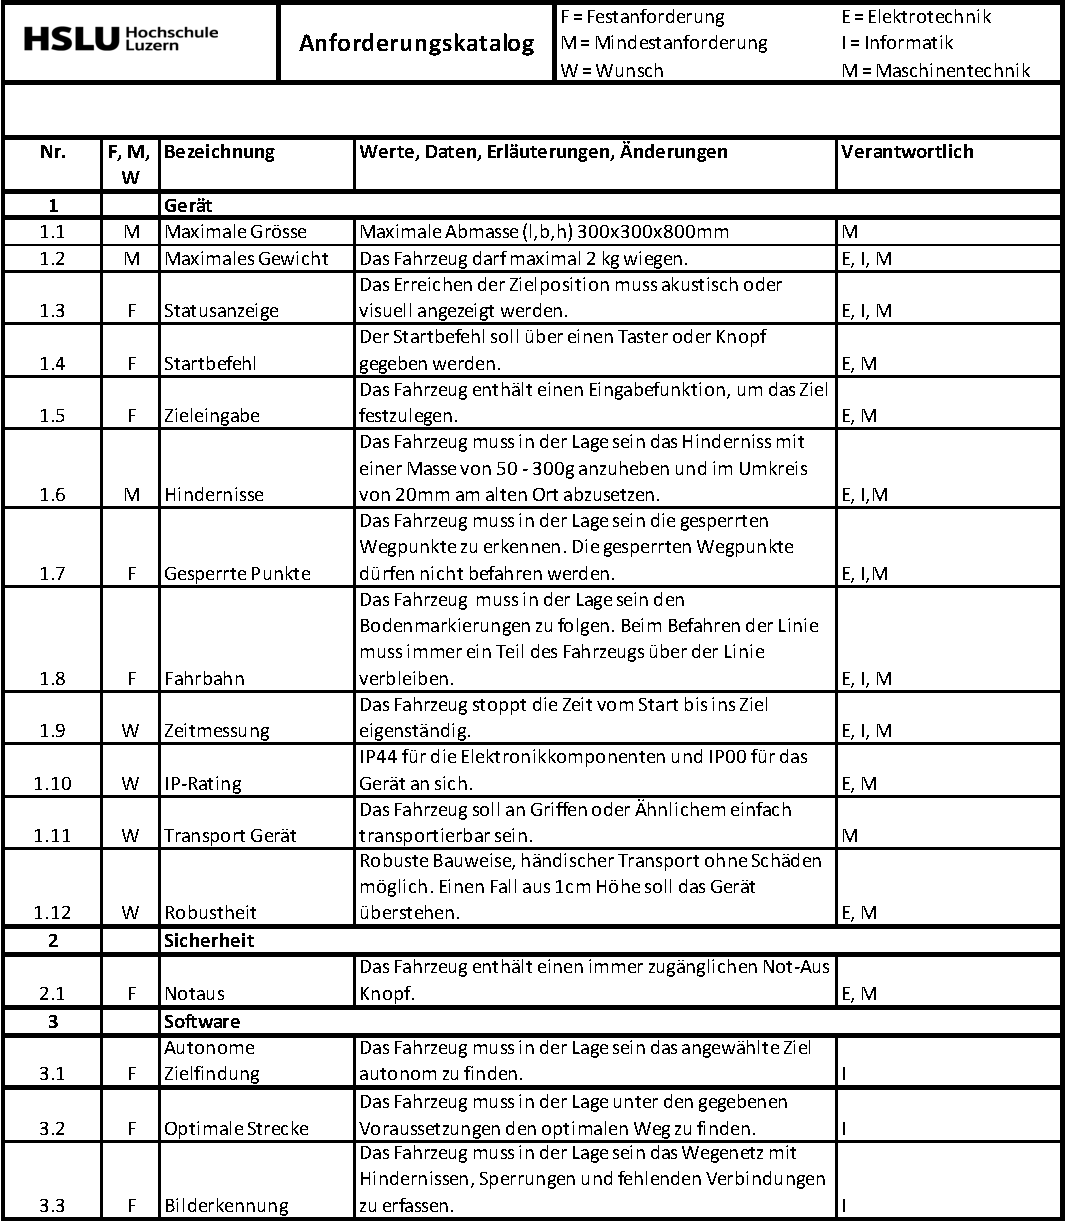
\includegraphics[width=\textwidth]{assets/Anforderungsliste_V1.01_page1.pdf}
\caption{Anforderungsliste Teil 1}
\label{table:anforderungsliste_page1}
\end{table}
\newpage

\begin{table}[H]
\centering
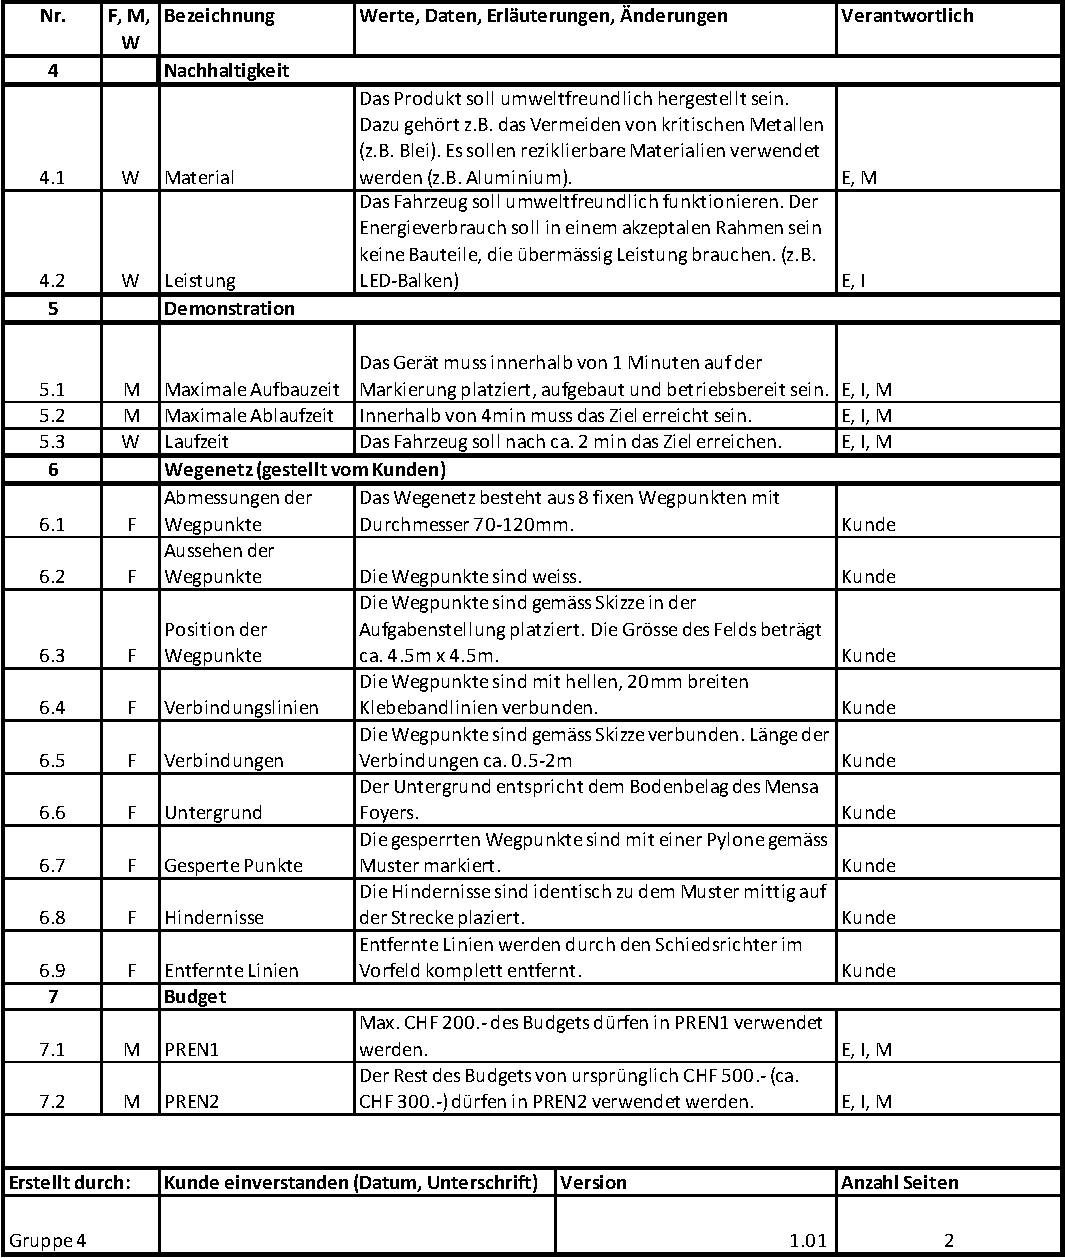
\includegraphics[width=\textwidth]{assets/Anforderungsliste_V1.01_page2.pdf}
\caption{Anforderungsliste Teil 2}
\label{table:anforderungsliste_page2}
\end{table}
\newpage

\begin{landscape}
\subsection*{Kommunikationsplan}\label{kommunikationsplan}
\addcontentsline{toc}{subsection}{Kommunikationsplan}

Die Kommunikationskanäle sind definiert wie gezeigt in Tabelle \ref{table:communications-plan}.

\begin{table}[H]
\centering
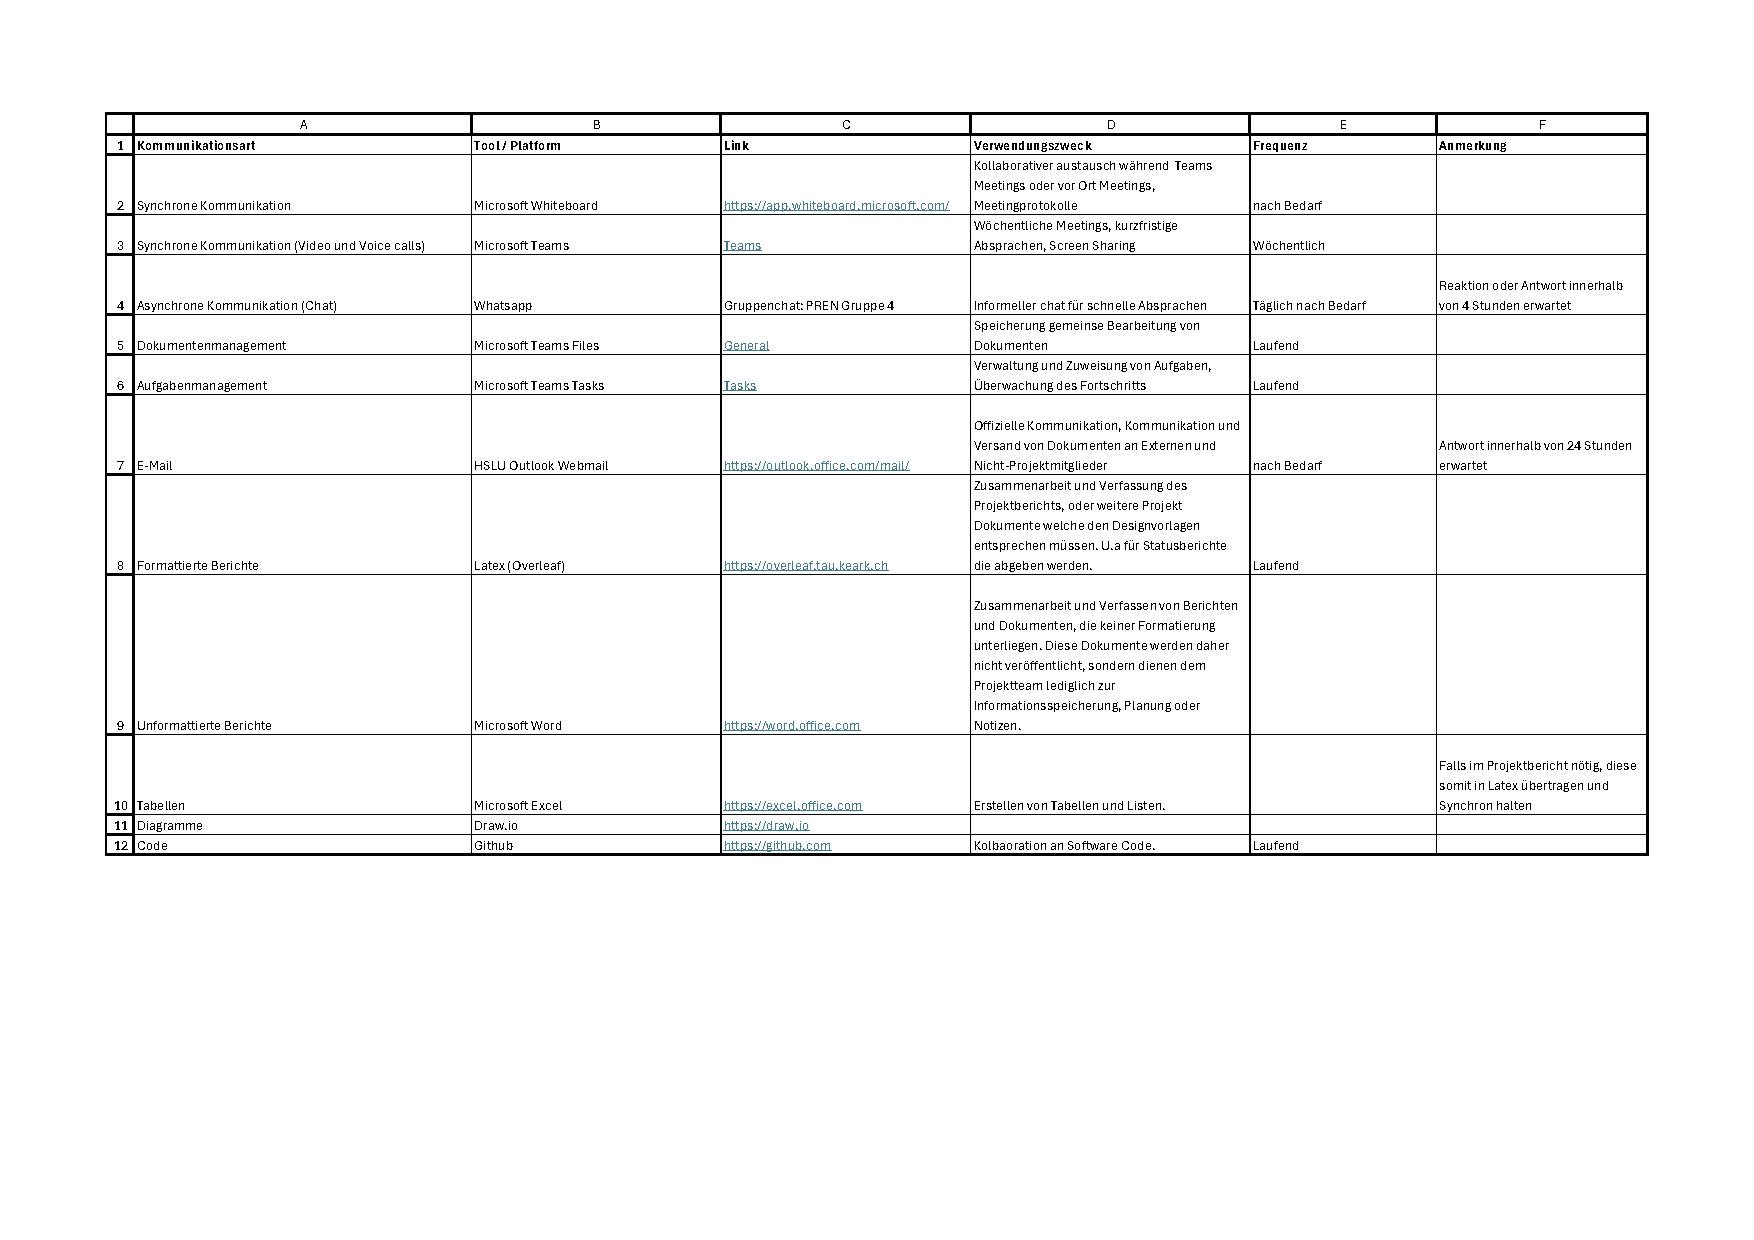
\includegraphics[width=240mm]{assets/Kommunikationschnittstellen.pdf}
\caption{Kommunikationsplan}
\label{table:communications-plan}
\end{table}
\end{landscape}

%%%%%%%%%%%%%%%%%% Technologierecherche %%%%%%%%%%%%%%%%%%%%

\subfile{parts/a-01-technologierecherchen}
\newpage

%%%%%%%%%%%%%%%%%%%%%% MK & Nutzwertanalysen %%%%%%%%%%%%%%%
\subfile{parts/a-02-konzept-varianten}
\newpage


%%%%%%%%% Prototyping %%%%%%%%%%%%%%
%%%%%%%%%%%%%%%%%%%%%%%%%%%%%%%%%%%%

\subfile{parts/a-02a-prototypen-mt}
\subfile{parts/a-02b-prototypen-et}
\subfile{parts/a-02c-prototypen-it}



%%% THIS IS USELESS %%%%%%%%%%%%

% \subsection{Originale Aufgabenstellung}\label{aufgabenstellung}

% Nachfolgend ist die originale Aufgabenstellung angehängt.

% 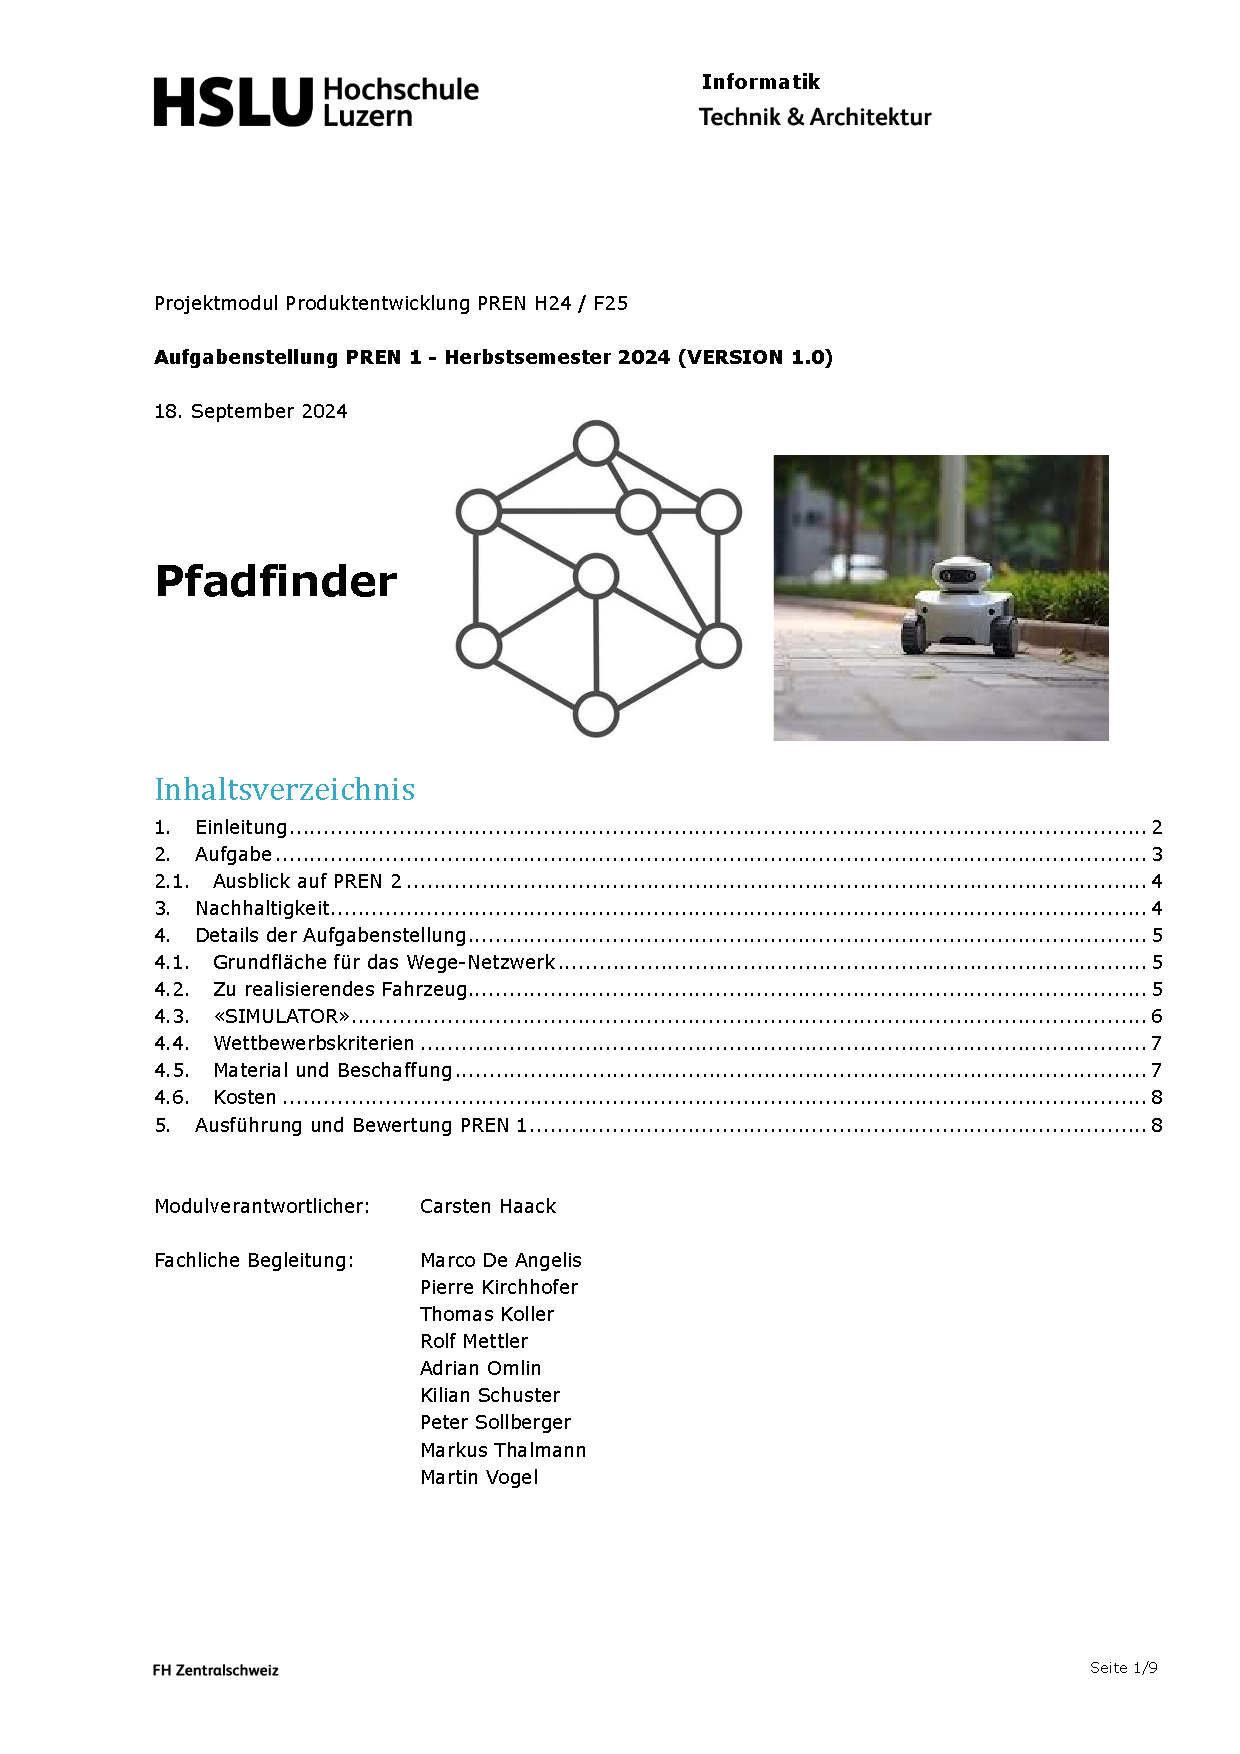
\includepdf[pages=-]{assets/AufgabenstellungPREN1HS24.pdf}
